\documentclass[aspectratio=169]{beamer} % [mathserif]
\usepackage{amsmath}
\usepackage{graphicx}
\usepackage{subfigure}
\usepackage{wrapfig}
\usepackage{booktabs}
\usepackage{hyperref}
\usepackage{media9}
% \usepackage{pgfplots}
% \pgfplotsset{compat=1.18}
% \usepgfplotslibrary{dateplot}
% \usepackage{tipa}
% \usepackage{epstopdf} % this is needed for windows Texworks
\usepackage[absolute,overlay]{textpos} % ,showboxes

\setlength{\TPHorizModule}{1in}
\TPVertModule=\TPHorizModule

\DeclareGraphicsExtensions{.eps}

\usetheme{Marburg}
% \usetheme{Berkeley}
% \usecolortheme{rose}
\definecolor{naublue}{HTML}{002454}
\definecolor{nauyellow}{HTML}{FAC01A}
%\setbeamercolor{structure}{bg=nauyellow, fg=naublue}
\setbeamercolor{palette primary}{bg=nauyellow, fg=naublue}
\setbeamercolor{palette secondary}{bg=nauyellow, fg=naublue}
%%%% See https://en.wikibooks.org/wiki/LaTeX/Presentations#User-defined_themes
% \setbeamercolor{alerted text}{fg=orange}
% \setbeamercolor{background canvas}{bg=white}
% \setbeamercolor{block body alerted}{bg=normal text.bg!90!black}
% \setbeamercolor{block body}{bg=normal text.bg!90!black}
% \setbeamercolor{block body example}{bg=normal text.bg!90!black}
% \setbeamercolor{block title alerted}{use={normal text,alerted text},fg=alerted text.fg!75!normal text.fg,bg=normal text.bg!75!black}
% \setbeamercolor{block title}{bg=blue}
% \setbeamercolor{block title example}{use={normal text,example text},fg=example text.fg!75!normal text.fg,bg=normal text.bg!75!black}
% \setbeamercolor{fine separation line}{}
\setbeamercolor{frametitle}{fg=naublue}
% \setbeamercolor{item projected}{fg=black}
% \setbeamercolor{normal text}{bg=black,fg=yellow}
% \setbeamercolor{palette sidebar primary}{use=normal text,fg=normal text.fg}
\setbeamercolor{palette sidebar primary}{bg=naublue, fg=nauyellow}
% \setbeamercolor{palette sidebar quaternary}{use=structure,fg=structure.fg}
% \setbeamercolor{palette sidebar secondary}{use=structure,fg=structure.fg}
% \setbeamercolor{palette sidebar tertiary}{use=normal text,fg=normal text.fg}
\setbeamercolor{section in sidebar}{fg=nauyellow, bg=naublue}
\setbeamercolor{section in sidebar shaded}{fg=white}
% \setbeamercolor{separation line}{}
% \setbeamercolor{sidebar}{bg=red}
% \setbeamercolor{sidebar}{parent=palette primary}
% \setbeamercolor{structure}{bg=black, fg=green}
% \setbeamercolor{subsection in sidebar}{fg=brown}
% \setbeamercolor{subsection in sidebar shaded}{fg=grey}
\setbeamercolor{title}{fg=naublue}
% \setbeamercolor{titlelike}{fg=brown}

% \usepackage[latin1]{inputenc}

%%%% See https://en.wikibooks.org/wiki/LaTeX/Presentations#Title_page_and_author_information
\title[INF632 (EE499/EE599)]{Wearable Technologies and Applications\\(Wearable Informatics)} %
\author{Winfree}
\date{Lecture 6}
%\institute{Northern Arizona University}

%\logo{\includegraphics[width=.5in]{figures/logo}}
% \setbeameroption{show notes on second screen}

\begin{document}
	\maketitle


% \section[Outline]{}
% \frame{\tableofcontents}

\section{Time-Series}
	\subsection{Last Time}
	\begin{frame}
		\frametitle{Comparing K-Means and KNN}
		Neither of these are great for time-series analysis.
		\begin{columns}
			\begin{column}{.5\linewidth}
				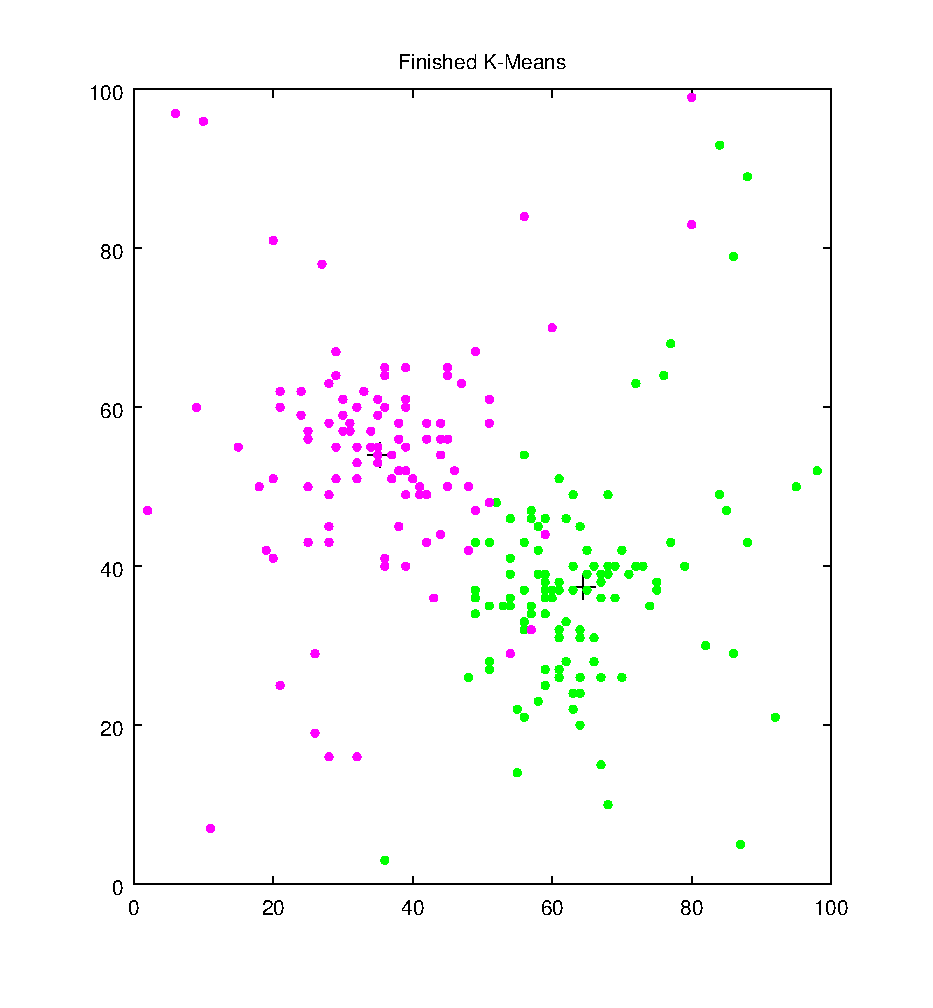
\includegraphics[width=.8\linewidth]{figures/kmeans_done.eps}

				K-Means pulls data apart, after you have the data.
			\end{column}
			\begin{column}{.5\linewidth}
				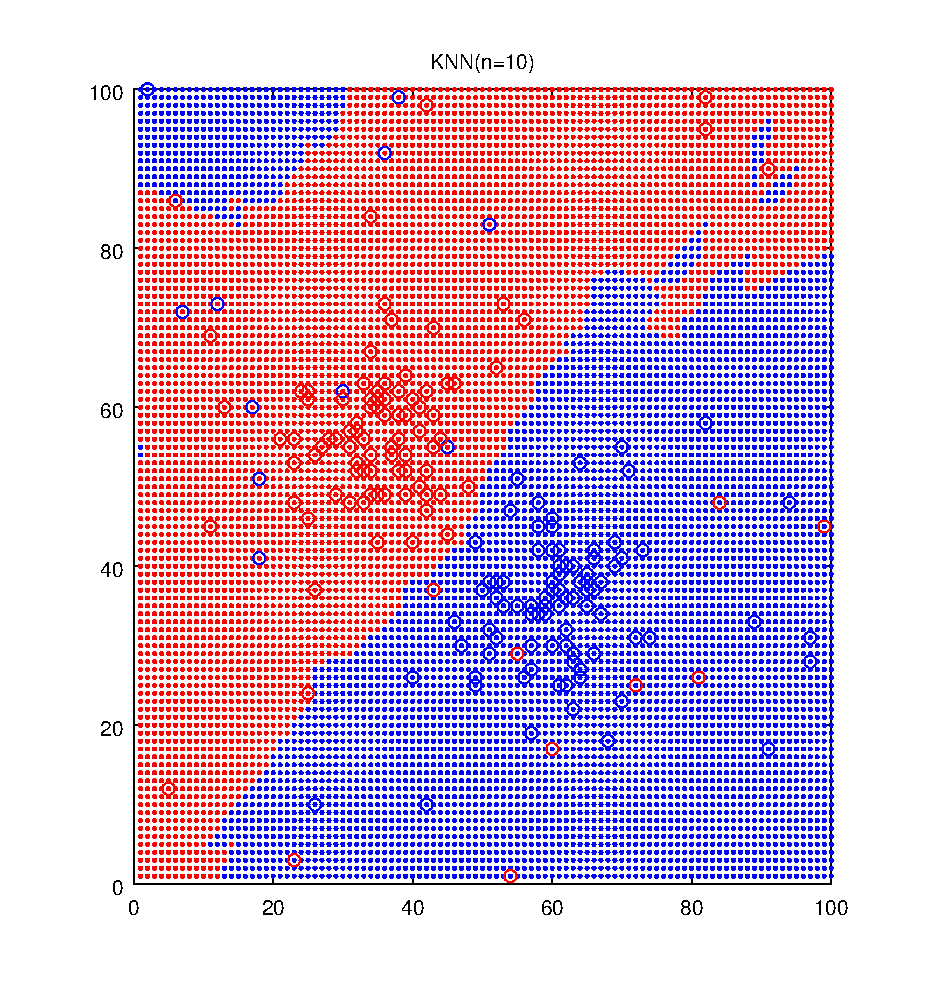
\includegraphics[width=.8\linewidth]{figures/KNN10.eps}

				Use the labeled data, can be used as a live model.
			\end{column}
		\end{columns}
		
	\end{frame}
	
	\subsection{X per Time Y}
	\begin{frame}
		\frametitle{Steps per Day}
		\begin{columns}
			\begin{column}{.5\linewidth}
				Suppose we have time series data
				\begin{itemize}
					\item Steps per day
					\item Steps per hour
					\item Heart rate per minute
				\end{itemize}
				You already looked at this in HW2, right?

				How did you approach that there?
			\end{column}
			\begin{column}{.5\linewidth}
				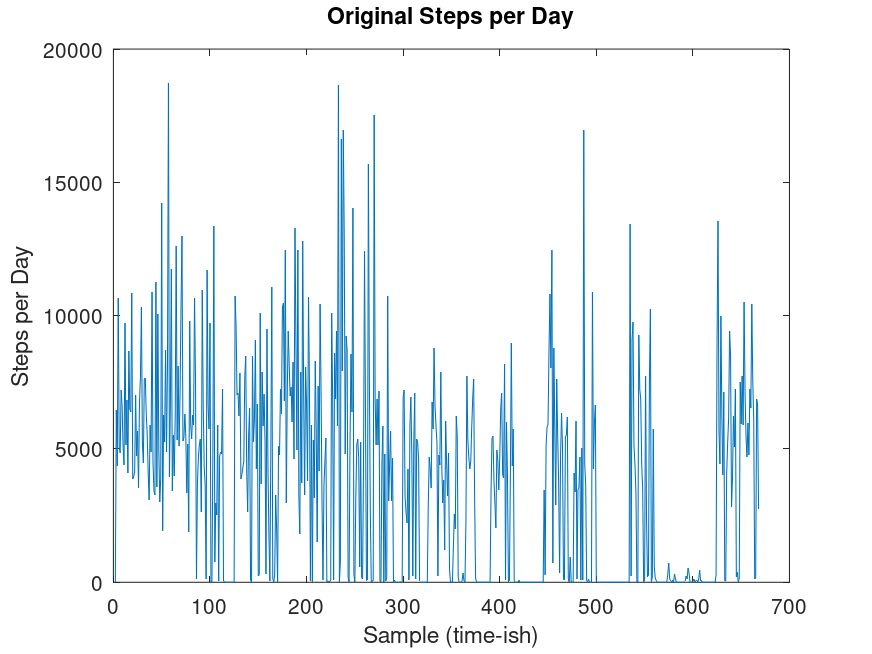
\includegraphics[width=1\linewidth]{figures/dailySteps.png}
			\end{column}
		\end{columns}
	\end{frame}

\section{Change Point Analysis}
	\subsection{Overview}
	\begin{frame}
	\frametitle{Overview}
		In statistical analysis, change detection or change point detection tries to identify times when the probability distribution of a stochastic process or time series changes. In general the problem concerns {\bf both} detecting {\em whether or not} a change has occurred, or whether several changes might have occurred, and {\em identifying the times of any such changes}.
		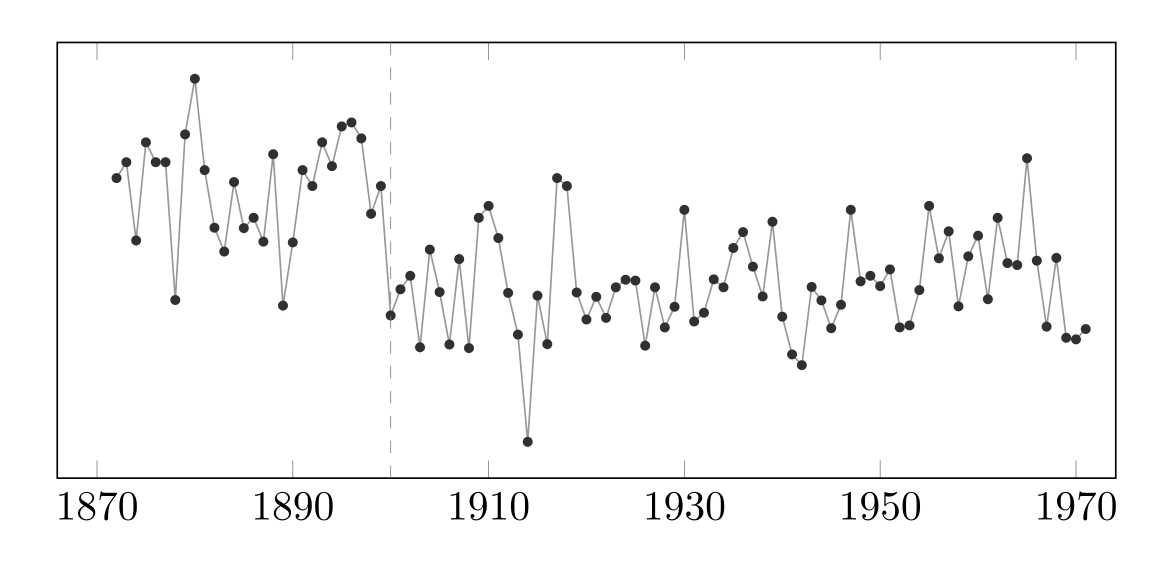
\includegraphics[width=1\linewidth]{figures/Nile_Discharge_Data.png}
		% Yearly volume of the Nile river at Aswan, an example of time series data commonly used in change detection. Dotted line denotes a detected change point when Old Aswan Dam was built in 1902.
	\end{frame}

	\begin{frame}
	\frametitle{Overview}
		% In statistical analysis, change detection or change point detection tries to identify times when the probability distribution of a stochastic process or time series changes. In general the problem concerns {\bf both} detecting {\em whether or not} a change has occurred, or whether several changes might have occurred, and {\em identifying the times of any such changes}.
		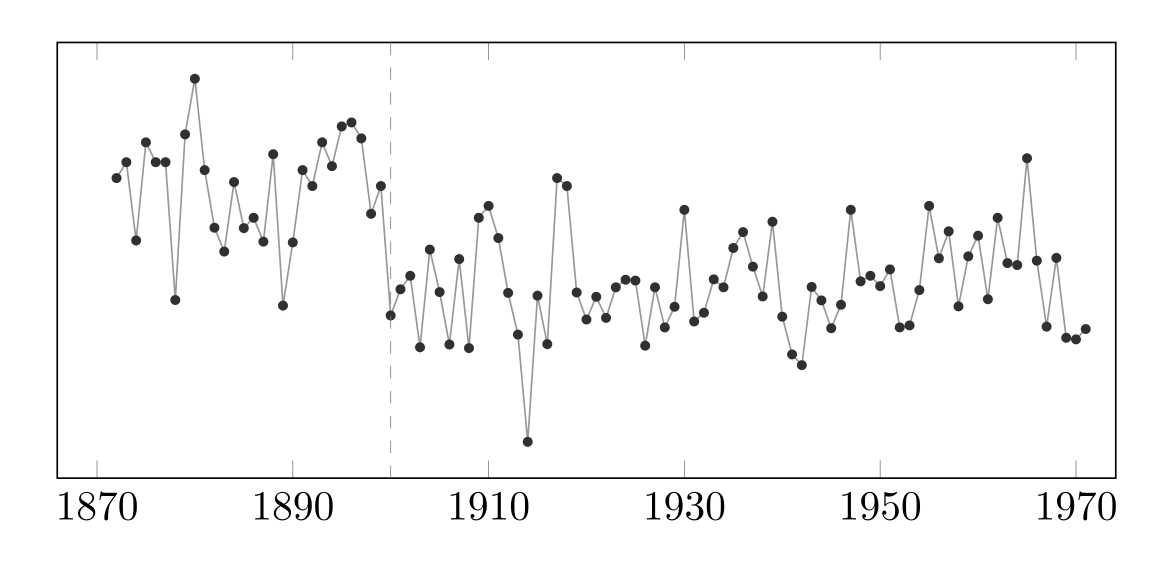
\includegraphics[width=1\linewidth]{figures/Nile_Discharge_Data.png}
		Yearly volume of the Nile river at Aswan, an example of time series data commonly used in change detection. Dotted line denotes a detected change point when Old Aswan Dam was built in 1902.
	\end{frame}

	\subsection{Algorithm}
	\begin{frame}
		\frametitle{Algorithm}
		\begin{columns}
			\begin{column}{.4\linewidth}
				\begin{align*}
					\vec{t} &= \mathrm{set~of~n~timestamps} \\
					\vec{x} &= \mathrm{set~of~n~measures} \\
				    % t_i &= \mathrm{ith~timestamp} \\
				    % x_i &= \mathrm{ith~measure} \\
				    \bar{x} &= \mathrm{mean~of~measures} \\
				    \vec{\varepsilon} &= x - \bar{x} = \mathrm{errors~from~mean} \\
				    y_i &= \sum_{j=i}^n \varepsilon_j \\
				    \vec{y} &= \mathrm{set~of~cumulative~sums} \\
				    R &= max(\vec{y}) - min(\vec{y}) \\
				    &= \mathrm{range}
				\end{align*}
			\end{column}
			\begin{column}{.6\linewidth}
				\begin{enumerate}
					\item Establish original cumulative sum ($\vec{y}$)
					\item Find / save $R_{original}$
					\item Find / save $i~\mathrm{of}~max(|\vec{y}|)$
					\item Bootstrap many times {\footnotesize ($K = 10 \ldots 1000$)}
						\begin{enumerate}
							\item Randomly re-order $x$
							\item Find / save new $\vec{y}$
						\end{enumerate}
					\item Find / save $R_{bootstraps}$
					\item Confidence $= \frac{\sum \left(R_{bootstraps} < R_{original}\right)}{K}$
					\item If Confidence $>$ some threshold,\\then $i~\mathrm{of}~max(|\vec{y}|)$ is CP
				\end{enumerate}
			\end{column}
		\end{columns}
	\end{frame}

\section{Example}
	\begin{frame}
		\frametitle{Example}
		\begin{columns}
			\begin{column}{.4\linewidth}
				How about that data again?

				~

				Let's ignore timestamps for this example.
			\end{column}
			\begin{column}{.6\linewidth}
				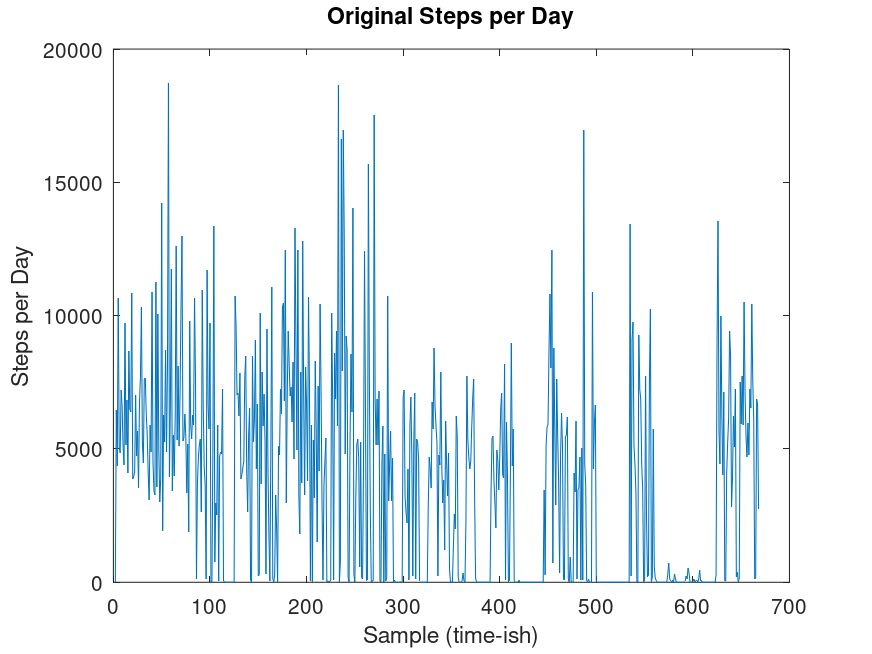
\includegraphics[width=1\linewidth]{figures/dailySteps.png}
			\end{column}
		\end{columns}
	\end{frame}
	\subsection{Validate and Clean Up}
	\begin{frame}
		\frametitle{Validate / Clean Up}
		\begin{columns}
			\begin{column}{.4\linewidth}
				Notice how we have some zero or near zero measures?

				~

				Let's assume those are times when the Fitbit wasn't being worn.
			\end{column}
			\begin{column}{.6\linewidth}
				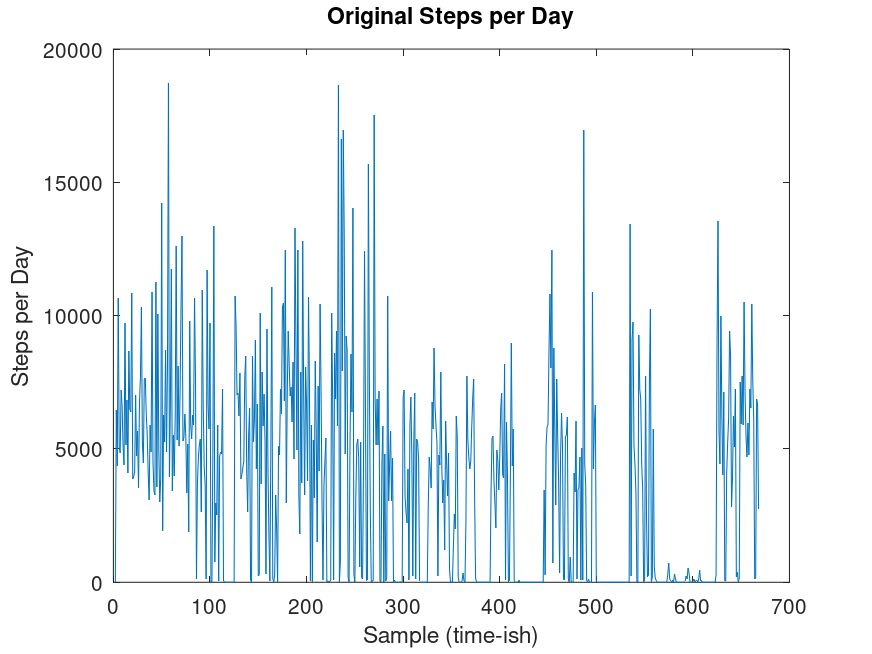
\includegraphics[width=1\linewidth]{figures/dailySteps.png}
			\end{column}
		\end{columns}
	\end{frame}

	\begin{frame}
		\frametitle{Validate / Clean Up}
		\begin{columns}
			\begin{column}{.4\linewidth}
				Notice how we have some zero or near zero measures?


				Let's assume those are times when the Fitbit wasn't being worn.

				We can sort these and plot, without regard for the timestamp.

				\centering
				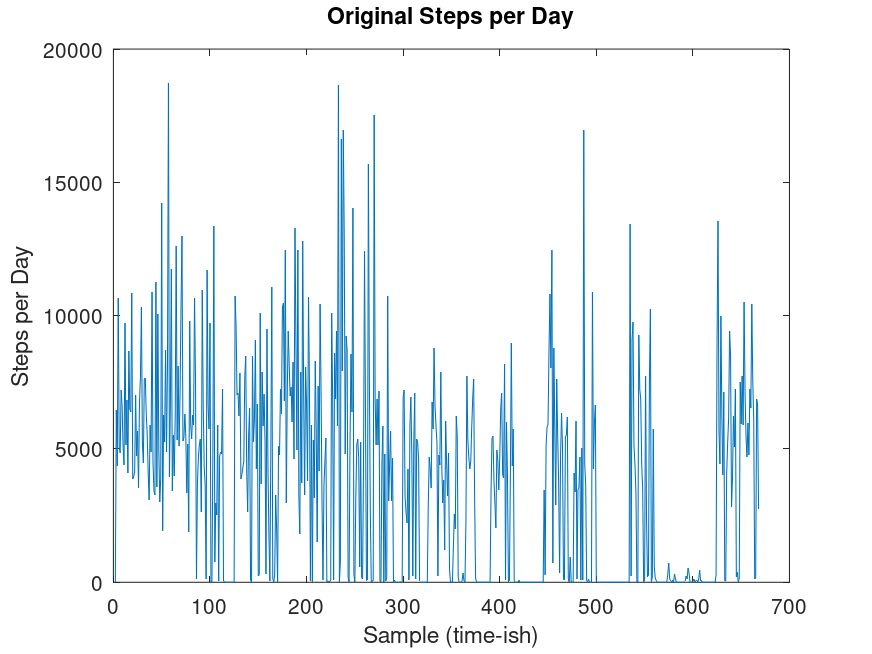
\includegraphics[width=.8\linewidth]{figures/dailySteps.png}
			\end{column}
			\begin{column}{.6\linewidth}
				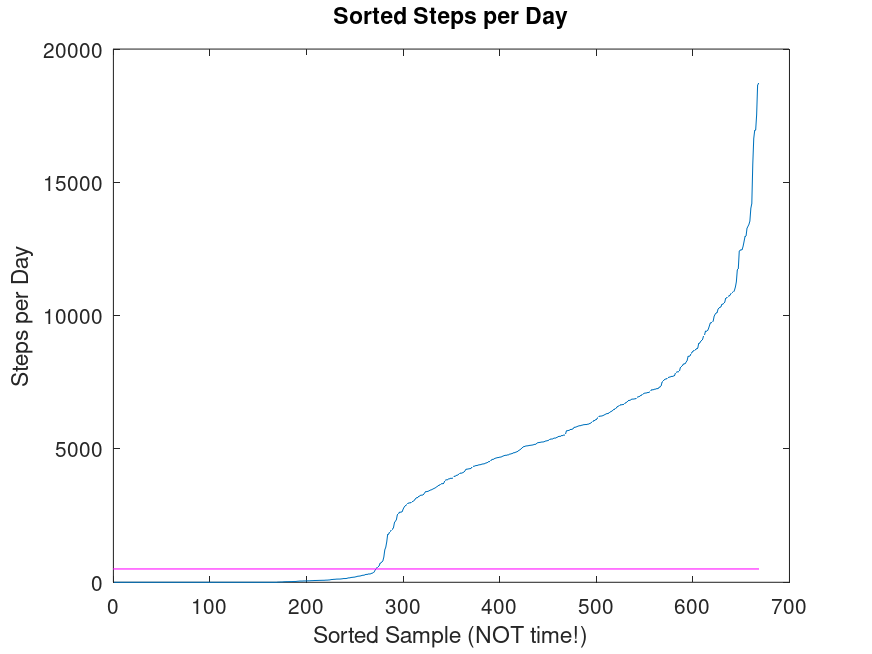
\includegraphics[width=1\linewidth]{figures/dailySteps_sorted.png}
			\end{column}
		\end{columns}
	\end{frame}

	\subsection{Subtract off the Mean}
	\begin{frame}
		\frametitle{Subtract off the Mean}
		\begin{columns}
			\begin{column}{.4\linewidth}
				With the ``off'' days out of the way, we can subtract the mean from all points.

				~ ~

				\centering
				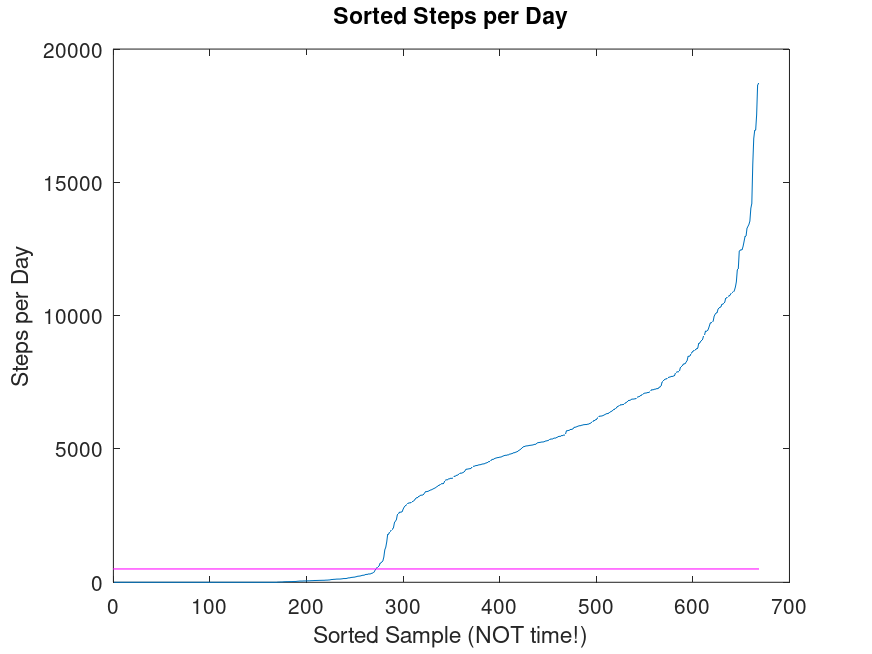
\includegraphics[width=.8\linewidth]{figures/dailySteps_sorted.png}
			\end{column}
			\begin{column}{.6\linewidth}
				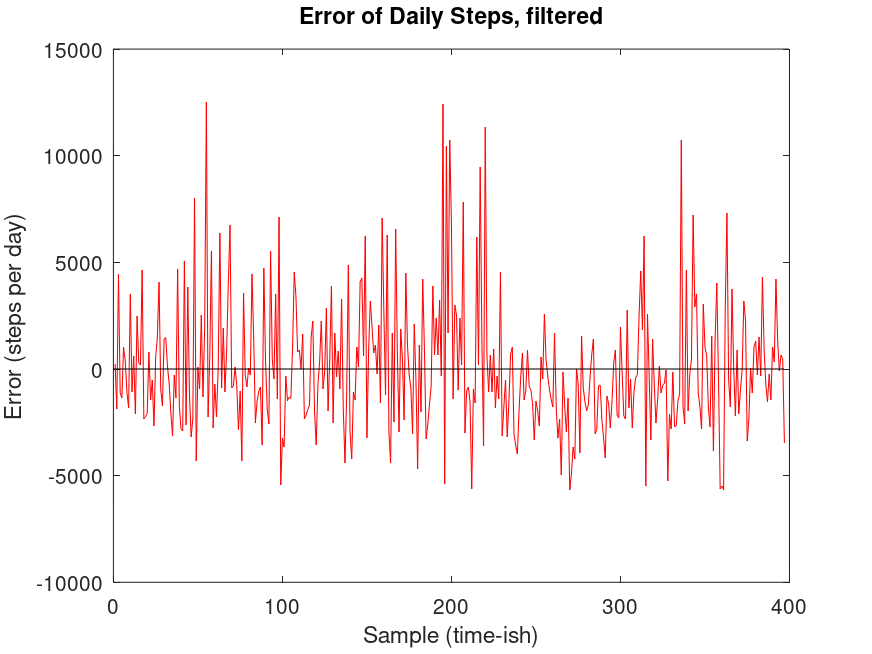
\includegraphics[width=1\linewidth]{figures/dailySteps_err.png}
			\end{column}
		\end{columns}
	\end{frame}

	\begin{frame}
		\frametitle{Subtract off the Mean}
		\begin{columns}
			\begin{column}{.4\linewidth}
				With the ``off'' days out of the way, we can subtract the mean from all points.

				Looks pretty similar, but ...

				\centering
				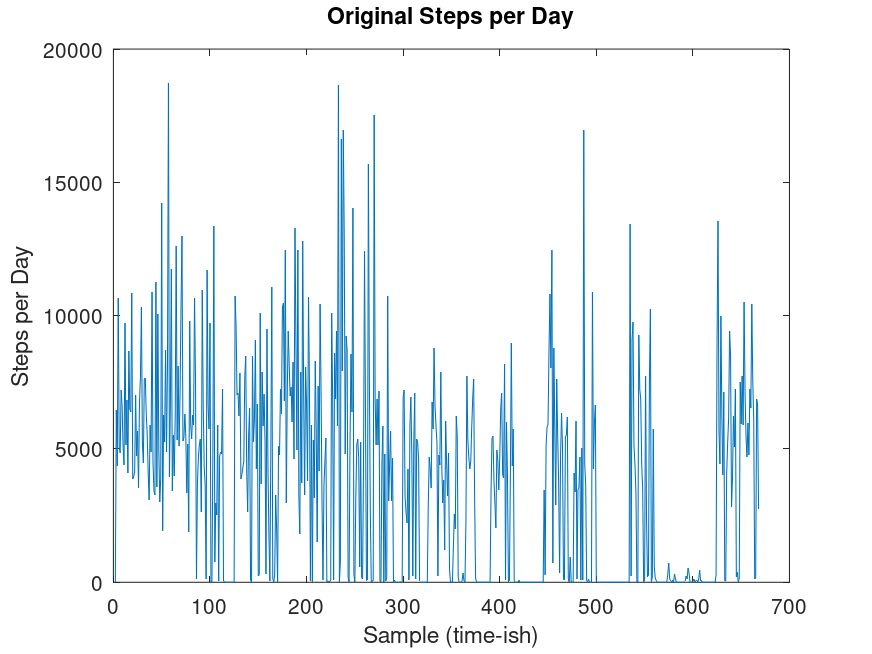
\includegraphics[width=.8\linewidth]{figures/dailySteps.png}
			\end{column}
			\begin{column}{.6\linewidth}
				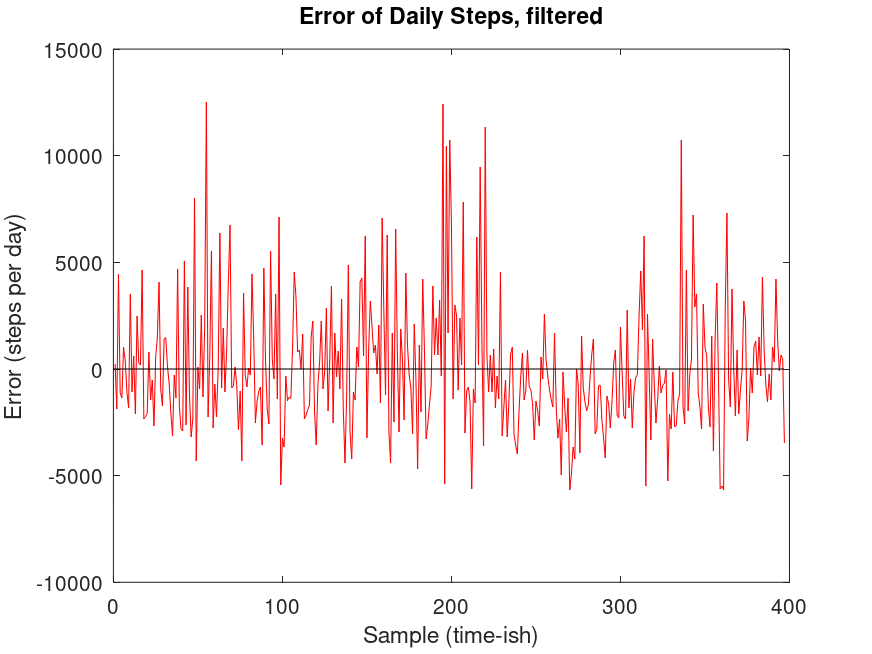
\includegraphics[width=1\linewidth]{figures/dailySteps_err.png}
			\end{column}
		\end{columns}
	\end{frame}

	\subsection{Cumulative Sum the Errors}
	\begin{frame}
		\frametitle{Subtract off the Mean}
		\begin{columns}
			\begin{column}{.4\linewidth}
				Calculate the cumulative sum of the errors, in the original data.

				See how this starts at zero and returns to zero?

				\centering
				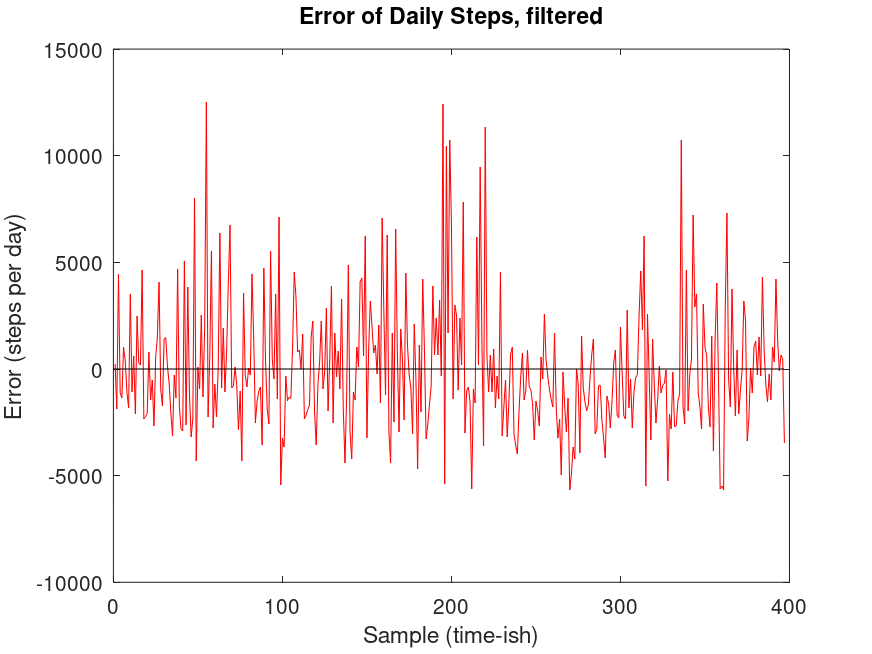
\includegraphics[width=.8\linewidth]{figures/dailySteps_err.png}
			\end{column}
			\begin{column}{.6\linewidth}
				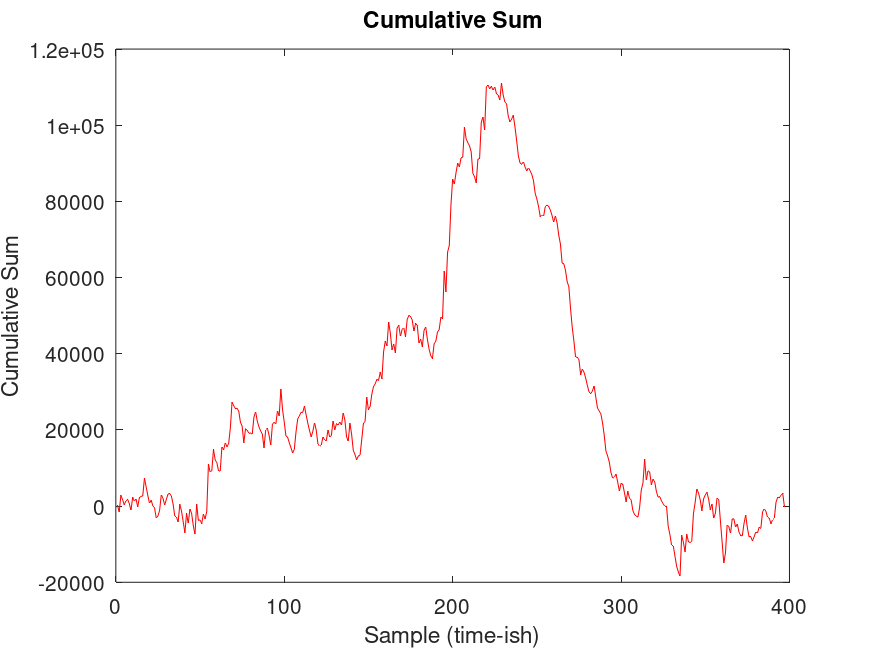
\includegraphics[width=1\linewidth]{figures/dailySteps_cumsum_err.png}
			\end{column}
		\end{columns}
	\end{frame}

	\subsection{Bootstrap it}
	\begin{frame}
		\frametitle{Bootstrap it}
		\begin{columns}
			\begin{column}{.4\linewidth}
				Randomize the order of the errors (or $x$ and then recalc $\varepsilon$).

				Calculate the cumulative sum of the errors.

				Do this ``many'' times.

				\centering
				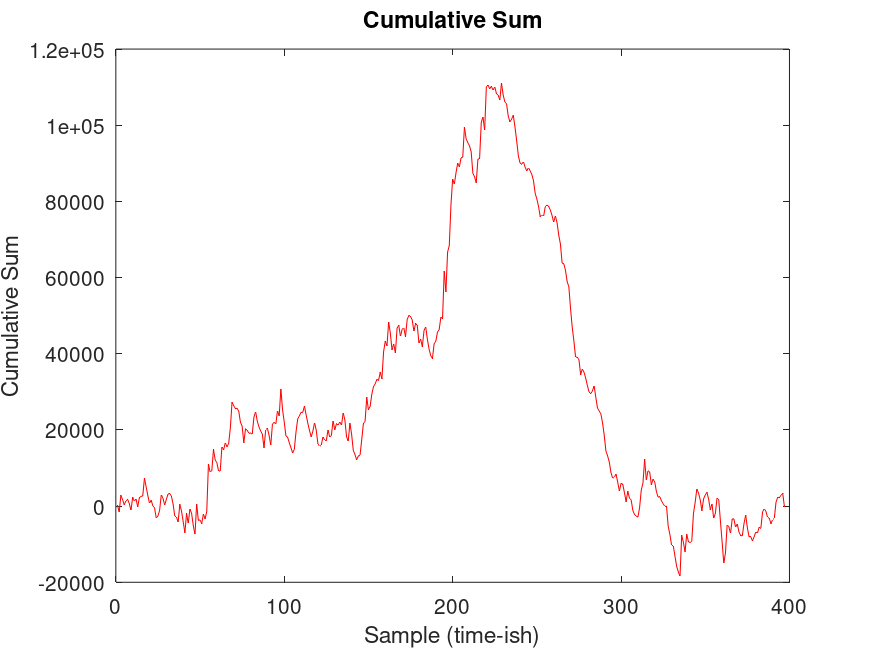
\includegraphics[width=.8\linewidth]{figures/dailySteps_cumsum_err.png}
			\end{column}
			\begin{column}{.6\linewidth}
				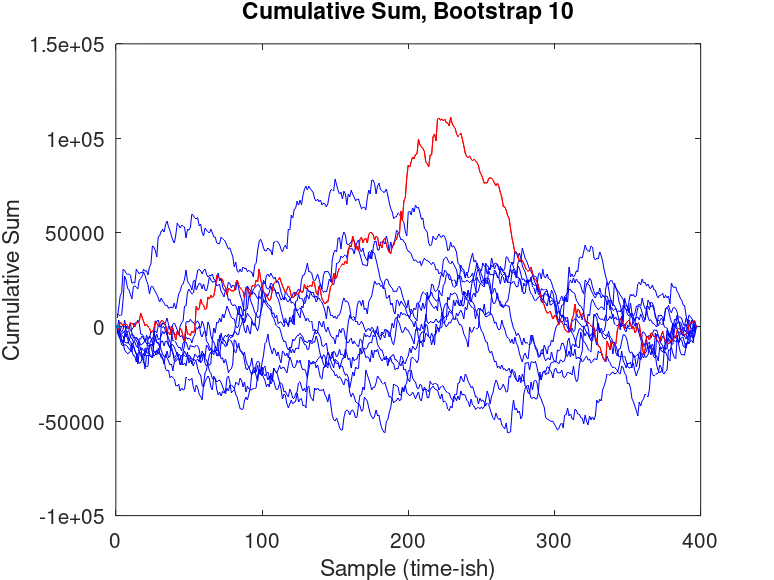
\includegraphics[width=1\linewidth]{figures/dailySteps_cumsum_err_bootstraped_10.png}
			\end{column}
		\end{columns}
	\end{frame}

	\subsection{Confidence}
	\begin{frame}
		\frametitle{Confidence}
		\begin{columns}
			\begin{column}{.4\linewidth}
				Statistically, how many times was the range of the original data larger than the bootstrapped reorders?

				Conf. $= \frac{\sum \left(R_{bootstraps} < R_{original}\right)}{K}$
				
				If Conf. $>$ some threshold,\\then $i~\mathrm{of}~max(|\vec{y}|)$ is change point!

				% \centering
				% 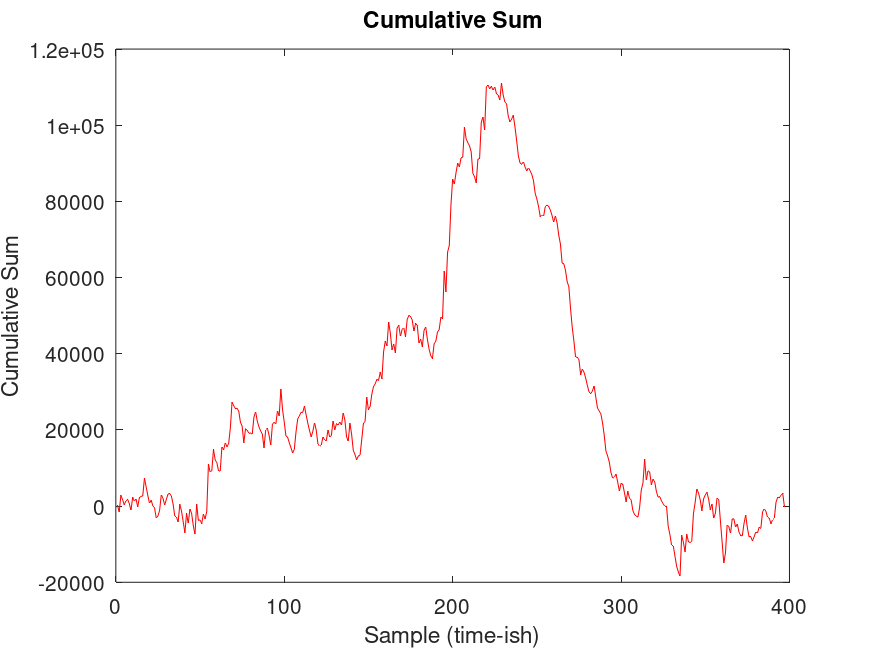
\includegraphics[width=.6\linewidth]{figures/dailySteps_cumsum_err.png}
			\end{column}
			\begin{column}{.6\linewidth}
				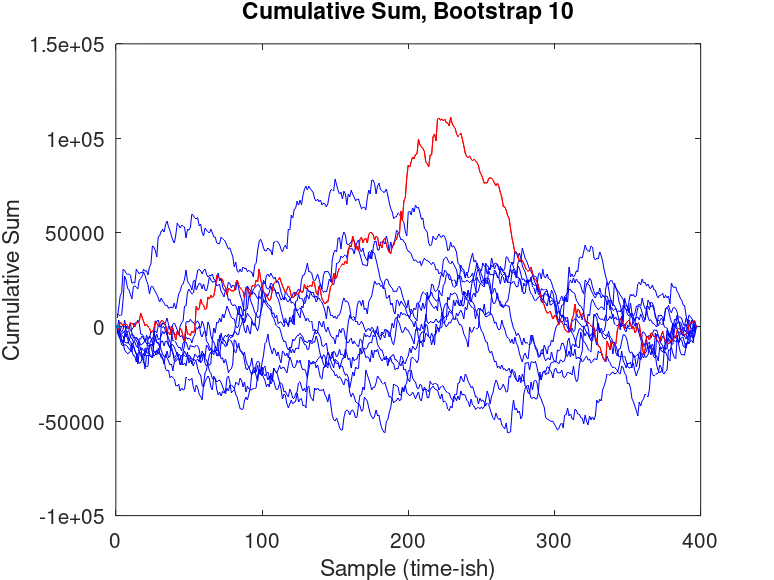
\includegraphics[width=1\linewidth]{figures/dailySteps_cumsum_err_bootstraped_10.png}
			\end{column}
		\end{columns}
	\end{frame}

	\subsection{Rinse and Repeat}
	\begin{frame}
		\frametitle{Rinse and Repeat}
		\begin{columns}
			\begin{column}{.4\linewidth}
				Because we found a change point, we need to cut the data in half and repeat this process on the left, and the right sections of data.

				\centering
				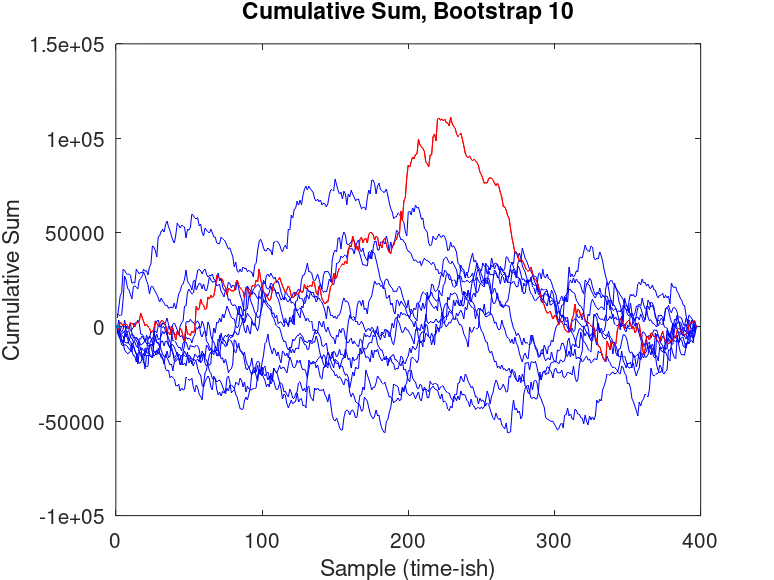
\includegraphics[width=.8\linewidth]{figures/dailySteps_cumsum_err_bootstraped_10.png}
			\end{column}
			\begin{column}{.6\linewidth}
				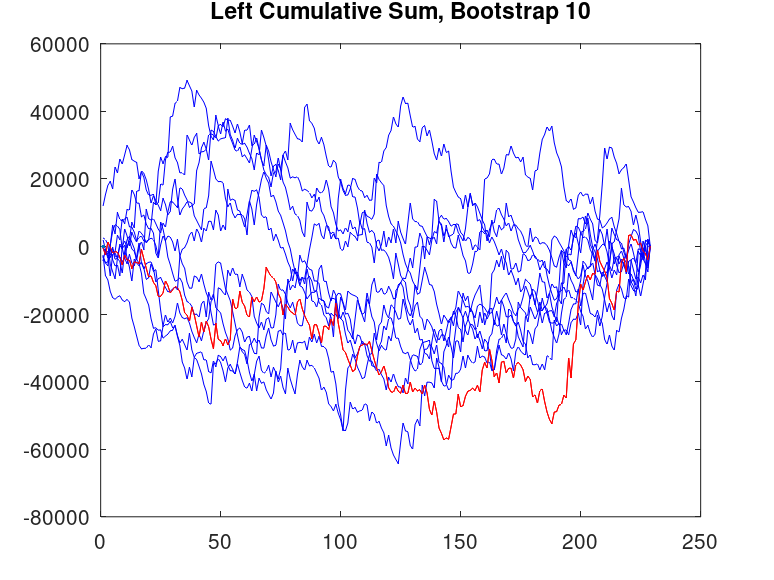
\includegraphics[width=1\linewidth]{figures/dailySteps_left_cumsum_err_bootstraped_10.png}
			\end{column}
		\end{columns}
	\end{frame}

\section{N Iterations}
	\subsection{10 vs 1000}
	\begin{frame}
		\frametitle{10 vs 1000}
		\begin{columns}
			\begin{column}{.4\linewidth}
				Best practice is to bootstrap some large number of times.  1000 is generally considered sufficient.  10, from our example, is {\em not}.

				\centering
				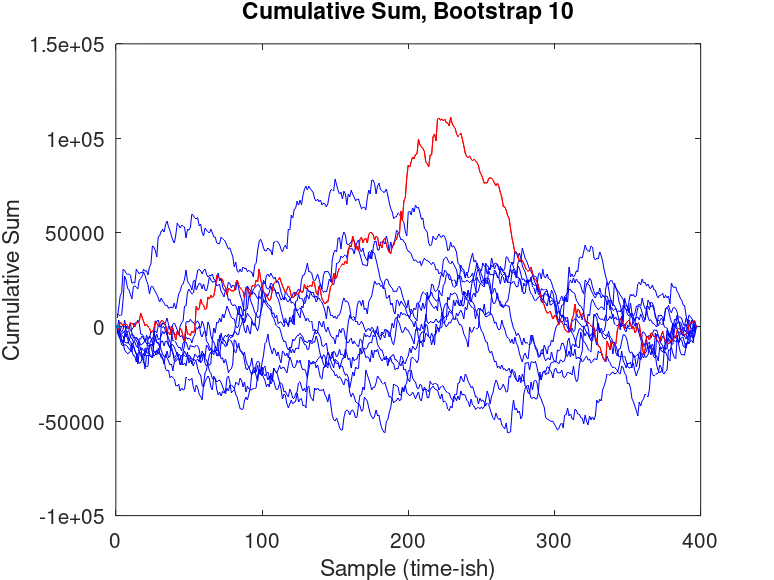
\includegraphics[width=.8\linewidth]{figures/dailySteps_cumsum_err_bootstraped_10.png}
			\end{column}
			\begin{column}{.6\linewidth}
				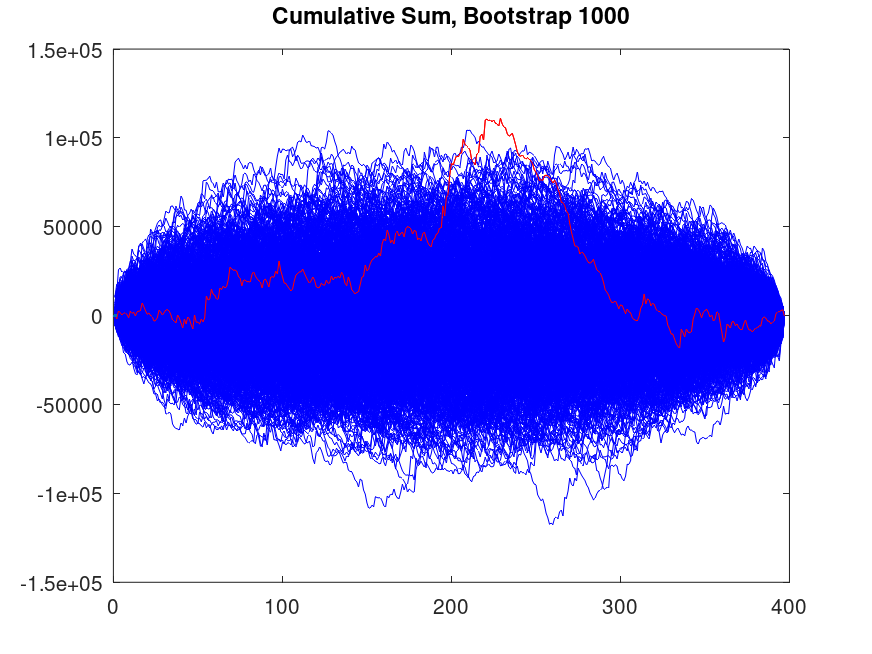
\includegraphics[width=1\linewidth]{figures/dailySteps_cumsum_err_bootstraped_1000.png}
			\end{column}
		\end{columns}
	\end{frame}


\end{document}
